\section{Data and methods}

\subsection{Station Selection}
The benchmark is constructed from the 3-hourly AntAWS station archive \citep{wang2023antaws}. The raw archive contains 267 station files after metadata matching and file-level screening. We retain stations only when they provide at least ten years of records, at least 70\% temperature completeness, at least 50\% mean completeness over the core variables, at least 20\% completeness for every core variable, and valid geographic metadata. Applied sequentially, these filters reduce the station pool from 267 to 117 after the record-length threshold, to 38 after the temperature-completeness threshold, to 36 after the core-mean threshold, and finally to 32 after the per-variable completeness threshold. The criteria remove stations that are long but effectively unusable for multivariate imputation, such as stations with nearly absent relative humidity records.

The final benchmark contains 32 stations. Twenty-seven stations are used for the main train/validation/test experiments, and five geographically separated stations are reserved for held-out generalization: Butcher Ridge, Mount Sidley, Nico, Sabrina, and Zhongshan. The held-out set was fixed before training by applying geographic farthest-point sampling to the eligible station set. It provides a station-level transfer test across separated Antarctic locations.

Table~\ref{tab:station-metadata} summarizes the selected station population. Appendix Table~\ref{tab:station-metadata-full} reports the full station-level metadata, temporal coverage, variable completeness, and split assignment.

\begin{table}[t]
  \centering
  \caption{Benchmark station summary. Completeness values are mean observed fractions over retained raw 3-hourly station records; full station metadata are reported in Appendix Table~\ref{tab:station-metadata-full}.}
  \label{tab:station-metadata}
  \begin{tabular}{lrrrrrr}
    \toprule
    Split & Stations & Years & Elev. & T & RH & q \\
    & & & (m) & (\%) & (\%) & (\%) \\
    \midrule
    held-out & 5 & 1989--2021 & 2030 & 78 & 82 & 70 \\
    main & 27 & 1984--2021 & 416 & 79 & 70 & 61 \\
    \bottomrule
  \end{tabular}
\end{table}


\subsection{ERA5 Alignment}
For each selected station, we download an ERA5 single-level point time series \citep{hersbach2020era5} using the CDS time-series API at the station latitude and longitude. The requested ERA5 variables are 2 m temperature, surface pressure, 2 m dewpoint temperature, and 10 m zonal and meridional wind. These variables are converted to the model channels used by AWS: temperature in $^\circ$C, relative humidity in percent, wind speed in m s$^{-1}$, pressure in hPa, and specific humidity in g kg$^{-1}$. Wind speed is computed from the two 10 m wind components. Relative humidity and specific humidity are derived from ERA5 temperature, dewpoint, and pressure using Bolton's saturation-vapor-pressure approximation \citep{bolton1980computation}, matching the AWS-derived humidity preprocessing.

The downloaded CDS point series is used as the ERA5 record for the station coordinates. The hourly ERA5 values are linearly interpolated to the exact AntAWS 3-hourly timestamps. All ERA5 files are checked for finite values and for matching temporal length before preprocessing. ERA5 and AWS channels are normalized with the same variable-wise statistics computed from main-station chronological training segments only. Held-out stations are excluded from those normalization statistics and from all model training.

In the benchmark windows, AWS observations define the target values at observed positions. The aligned ERA5 sequence is stored as an external meteorological background for the same timestamps.

AWS specific humidity is derived during preprocessing from temperature, relative humidity, and pressure using the same saturation-vapor-pressure formula and is stored in g kg$^{-1}$. Its observation mask is the intersection of the source-variable masks: if any required source value is missing or non-finite, the derived $q$ value is marked missing. Artificial masks are sampled after this derivation on the five-channel benchmark representation. The ERA5 $q$ channel is aligned and normalized with the same train-window statistics as the AWS-derived $q$ target.

\subsection{Sparse Window Generation}
Strictly complete windows are rare in Antarctic AWS records. Requiring every variable to be observed for a full 168-step window would leave few windows and bias the benchmark toward unusually clean periods, so windows are generated with explicit observation masks.

Each window contains $T=168$ 3-hourly steps, corresponding to three weeks. The preprocessing stride is 42 steps, or one quarter of the window length. Windows are retained when at least 25\% of all variable-time positions are observed, at least three variables have at least 12 observed steps inside the window, and the station belongs to the selected main or held-out split. Within each station, retained windows are ordered chronologically and assigned to 70\% train, 10\% validation, and 20\% test segments. The final preprocessing output contains 41,388 windows with normalized AWS values, binary observation masks, aligned ERA5 sequences, timestamp encodings, start indices, start timestamps, and split identifiers. Artificial masks are sampled from observed positions in this window representation.

Table~\ref{tab:split-overlap-audit} reports the chronological split gaps and sliding-window overlap. For every station, the validation segment lies between the training and test segments; the minimum train--test gap is 2268 steps, which is much longer than the 168-step input window. Validation and test windows can overlap because windows are generated with a 42-step stride. We also define a deterministic non-overlapping test subset by retaining test windows with start times separated by at least 168 steps. This subset contains 2102 windows, or 25.3\% of the original test windows.

\begin{table}[t]
  \centering
  \caption{Chronological split-overlap audit. Gaps are measured between the end of the earlier split window and the start of the later split window within each station. Negative values indicate context overlap. The non-overlap subset greedily retains test windows separated by at least one 168-step window length.}
  \label{tab:split-overlap-audit}
  \footnotesize
  \setlength{\tabcolsep}{3pt}
  \begin{tabular}{@{}p{0.36\linewidth}p{0.39\linewidth}p{0.18\linewidth}@{}}
    \toprule
    Quantity & Value & Stations \\
    \midrule
    Test windows & 8307 & 32 \\
    Non-overlap subset & 2102 (25.3\%) & 32 \\
    Test stride & median 42 steps & 32 \\
    Train--test gap & min 2268; median 4767 steps & 0 overlap \\
    Val--test gap & min -126; median -126 steps & 32 overlap \\
    \bottomrule
  \end{tabular}
\end{table}


\subsection{Observed Missingness}
The selected records contain many contiguous gaps. Wind speed and relative humidity carry the largest missing burden, with 90th-percentile gap lengths exceeding two days (Fig.~\ref{fig:missing-patterns}). This pattern motivates block-wise artificial masks for the main experiments. The observed mask records which AWS values are available in each sparse window.

\begin{figure}[t]
  \centering
  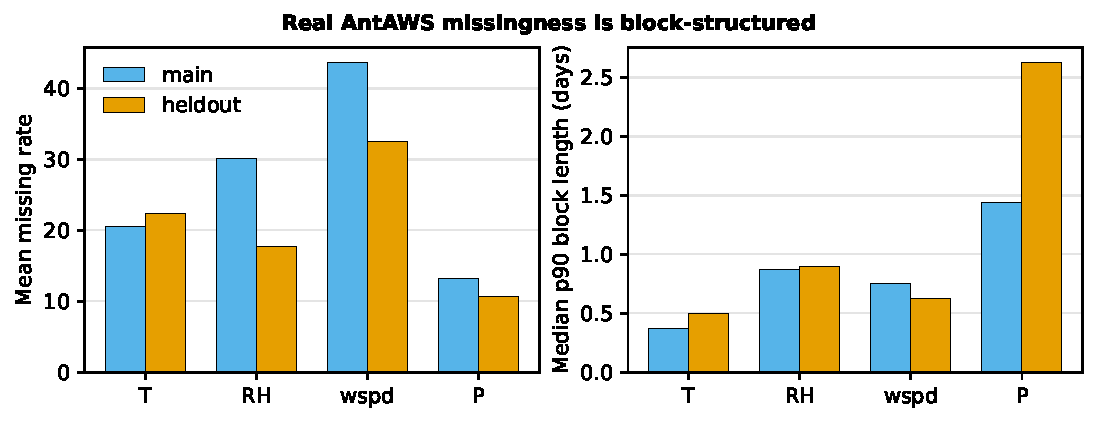
\includegraphics[width=\columnwidth]{figures/fig_missing_patterns.pdf}
  \caption{Observed missingness in selected AntAWS stations. Wind speed and relative humidity show the largest missing burden, and high-percentile gaps last multiple days, motivating block-wise rather than point-wise imputation.}
  \label{fig:missing-patterns}
\end{figure}
